%% LyX 2.1.2 created this file.  For more info, see http://www.lyx.org/.
%% Do not edit unless you really know what you are doing.
\documentclass[a4paper]{article}
\usepackage[latin9]{inputenc}
\usepackage{color}
\usepackage{array}
\usepackage{verbatim}
\usepackage{amsmath}
\usepackage{graphicx}
\usepackage[unicode=true]
 {hyperref}
\usepackage{breakurl}

\makeatletter

%%%%%%%%%%%%%%%%%%%%%%%%%%%%%% LyX specific LaTeX commands.
\special{papersize=\the\paperwidth,\the\paperheight}

%% Because html converters don't know tabularnewline
\providecommand{\tabularnewline}{\\}

%%%%%%%%%%%%%%%%%%%%%%%%%%%%%% User specified LaTeX commands.
% Template for EUSIPCO 2015 paper; to be used with:
%          spconf.sty  - LaTeX style file, and
%          IEEEbib.bst - IEEE bibliography style file.
% --------------------------------------------------------------------------
\usepackage{spconf}
\usepackage{graphicx}
\usepackage{cite}
\usepackage{xcolor}
\selectcolormodel{gray}

% Example definitions.
% --------------------
\def\x{{\mathbf x}}
\def\L{{\cal L}}

% Title.
% ------
\title{On the use of lyrical duration from musical score for automatic lyrics-to-audio alignment}
%
% Single address.
% ---------------
\name{Georgi Dzhambazov, Xavier Serra}
%\address{Author Affiliation(s)}
%
% For example:
% ------------
\address{Music Technology Group\\
Universitat Pompeu Fabra\\
Barcelona}
%
% Two addresses (uncomment and modify for two-address case).
% ----------------------------------------------------------
%\twoauthors
%  {A. Author-one, B. Author-two\sthanks{Thanks to XYZ agency for funding.}}
%	{School A-B\\
%	Department A-B\\
%	Address A-B}
%  {C. Author-three, D. Author-four\sthanks{The fourth author performed the work
%	while at ...}}
%	{School C-D\\
%	Department C-D\\
%	Address C-D}
%
% Multiple author/addresses combination (use only in particular cases).
% ---------------------------------------------------------------------
%\name{A. Author-one$^*$, B. Author-two$^*$$^\dagger$, C. Author-three$^\dagger$, D. Author-four$^\ddagger$ %
%	\thanks{General thanks/acknowledgment}%
%	\thanks{$^*$ Thanks/acknowledgments for authors marked with *}%
%	\thanks{$^\dagger$ Thanks/acknowledgments for authors marked with $\dagger$}%
%	\thanks{$^\ddaggerstitute ABC\\
%		Group Group ABC\\
%		Address ABC
%	\endtabular$ Thanks/acknowledgments for authors marked with $\ddagger$}%
%}
%\address{%
%    \tabular{c}
%		$^*$ In
%	\hskip 0.5in
%    \tabular{c}
%		$^\dagger$ School DEF\\
%		Department DEF\\
%		Address DEF
%	\endtabular
%	\hskip 0.5in
%    \tabular{c}
%		$^\ddagger$ Company GHI\\
%		Department GHI\\
%		Address GHI
%	\endtabular
%}
%
% The symbol order for multiple author combination is:
%  $^*$, $^\dagger$, $^\ddagger$, $^\mathsection$, $^\mathparagraph$, $^\|$,
%  $^{**}$, $^{\dagger\dagger}$, $^{\ddagger\ddagger}$, ...
%
%
% Alternative multiple author/addresses combination (use only in particular cases).
% ---------------------------------------------------------------------------------
%\name{A. Author-one$^*$, B. Author-two$^*$$^\dagger$, C. Author-three$^\dagger$, D. Author-four$^\ddagger$ %
%	\thanks{General thanks/acknowledgment}%
%	\thanks{$^*$ Thanks/acknowledgments for authors marked with *}%
%	\thanks{$^\dagger$ Thanks/acknowledgments for authors marked with $\dagger$}%
%	\thanks{$^\ddagger$ Thanks/acknowledgments for authors marked with $\ddagger$}%
%}
%\address{%
%	$^*$ Institute ABC, Group Group ABC, Address ABC\\
%	$^\dagger$ School DEF, Department DEF, Address DEF\\
%	$^\ddagger$ Company GHI, Department GHI, Address GHI\\
%}
%
% The symbol order for multiple author combination is:
%  $^*$, $^\dagger$, $^\ddagger$, $^\mathsection$, $^\mathparagraph$, $^\|$,
%  $^{**}$, $^{\dagger\dagger}$, $^{\ddagger\ddagger}$, ...
%

\makeatother

\begin{document}
\maketitle 
\begin{abstract}
In this work we show that automatic lyrics-to-audio alignment can
be improved by explicitly modeling sung vocal durations. The system
is a variant of a duration-explicit hidden Markov model (DHMM) phonetic
recognizer based on timbral features: mel frequency cepstral coefficients
(MFCCs). We modify the standard scheme for text-to-speech alignment
to address the differences of phoneme durations, specific for singing.
Phoneme durations are inferred from sheet music.

The proposed approach is tested on polyphonic audio from the classical
Turkish music tradition, whereby MFCCs are extracted in a way robust
to background instrumental sounds. In order to assess the impact of
the polyphonic setting, alignment is evaluated as well on an acapella
dataset, compiled especially for this study.

We show that the inclusion of duration information improves alignment
accuracy by absolute 10 percent on the level of lyrics lines (phrases)
and performs on par with state-of-the-art aligners for other languages.
\end{abstract}
\begin{keywords} lyrics-to-audio alignment; score-informed alignment;
phoneme durations; singing voice tracking; Turkish classical music\end{keywords} 


\section{Introduction}

\label{sec:intro}

The automatic synchronization between lyrics and audio is a challenging
research problem. \textcolor{red}{}It has inherent relation to text-to-speech
alignment. For spoken utterances phonemes have relatively similar
duration across speakers. Unlike that, in singing durations of phoneme
(especially vowels) have higher variation \cite{kruspekeyword}. When
being sung, vowels are prolonged according to musical note values,
which in term have intrinsic relation to musical meter (e.g. duration
could align with beats in a musical bar). 

Another aspect that distinguishes speech from music is that unlike
clean speech, singing voice is accompanied by background instruments.
Instrumental accompaniment and non-vocal segments can deteriorate
significantly the alignment accuracy.

The goal of this study is to test the hypothesis that extending a
state-of-the-art system for automatic lyrics-to-audio alignment with
modeling of phoneme durations, can improve its accuracy. More specifically,
we aim to show that durations of vocals (inferred from musical score)
can guide the recognition process in cases when it looses track in
polyphonic audio. Such guidance can be compared to the way modeling
prosodic rules helps in automatic speech understanding. 

While being aided by sheet music, our modeling approach allows at
the same time room for certain temporal flexibility to handle cases
of expressive singing, in which vocals are sustained in a way not
obeying the reference sheet music. The proposed approach was tested
on polyphonic audio from the classical Turkish tradition which is
characterized by high degree of expressive singing, thus providing
challenging material with versatile temporal deviations.  


\section{Related Work}

To date most of the studies of automatic lyrics-to-audio alignment
exploit phonetic acoustic features and state-of-the-art work is based
on a phoneme recognizer \cite{fujihara2011lyricsynchronizer,Mesaros96automaticalignment}.

An example of such a system \cite{fujihara2011lyricsynchronizer}
relies on hidden Markov model (HMM) and was tested on Japanese popular
music. To reduce the spectral content of background instruments, the
authors perform automatic segregation of the vocal line. Then Viterbi
forced alignment \cite{rabiner1989tutorial} is run utilizing mel
frequency cepstral coefficients (MFCCs) extracted from the vocal-only
signal. In both \cite{fujihara2011lyricsynchronizer} and \cite{Mesaros96automaticalignment}
the phoneme models are trained on speech and later adapted to singing
voice. This is necessary because of the lack of big enough training
singing voice corpus. In \cite{fujihara2011lyricsynchronizer} additionally
an adaptation to the voice of a particular singer is carried out.


In other works duration of lyrics has been applied as a reinforcing
cue: In \cite{wang2004lyrically} relative estimated durations are
inferred directly from textual lyrics. The estimation process is done
based on supervised training on singing voice. 

\begin{comment}
how to model duration 
\end{comment}


A common-occurring drawback of HMMs is that their capability to model
exact state durations is restricted. The wait time in a state is implicitly
set to a geometric distribution (derived from the self-transition
likelihood). Duration is usually modeled by duration-explicit hidden
Markov models (DHMM) (a.k.a. hidden semi-Markov models). In DHMMs
the underlying process is allowed to be a semi-Markov chain with variable
duration of each state \cite{yu2010hidden}. Each state in turn can
be assigned any statistical distribution. DHMMs have been shown to
be successful for modeling chord durations in automatic chord recognition
\cite{chen2012chord}. 


\section{Proposed System}

\begin{figure}
\begin{minipage}[b]{1\linewidth}%
\centering  \centerline{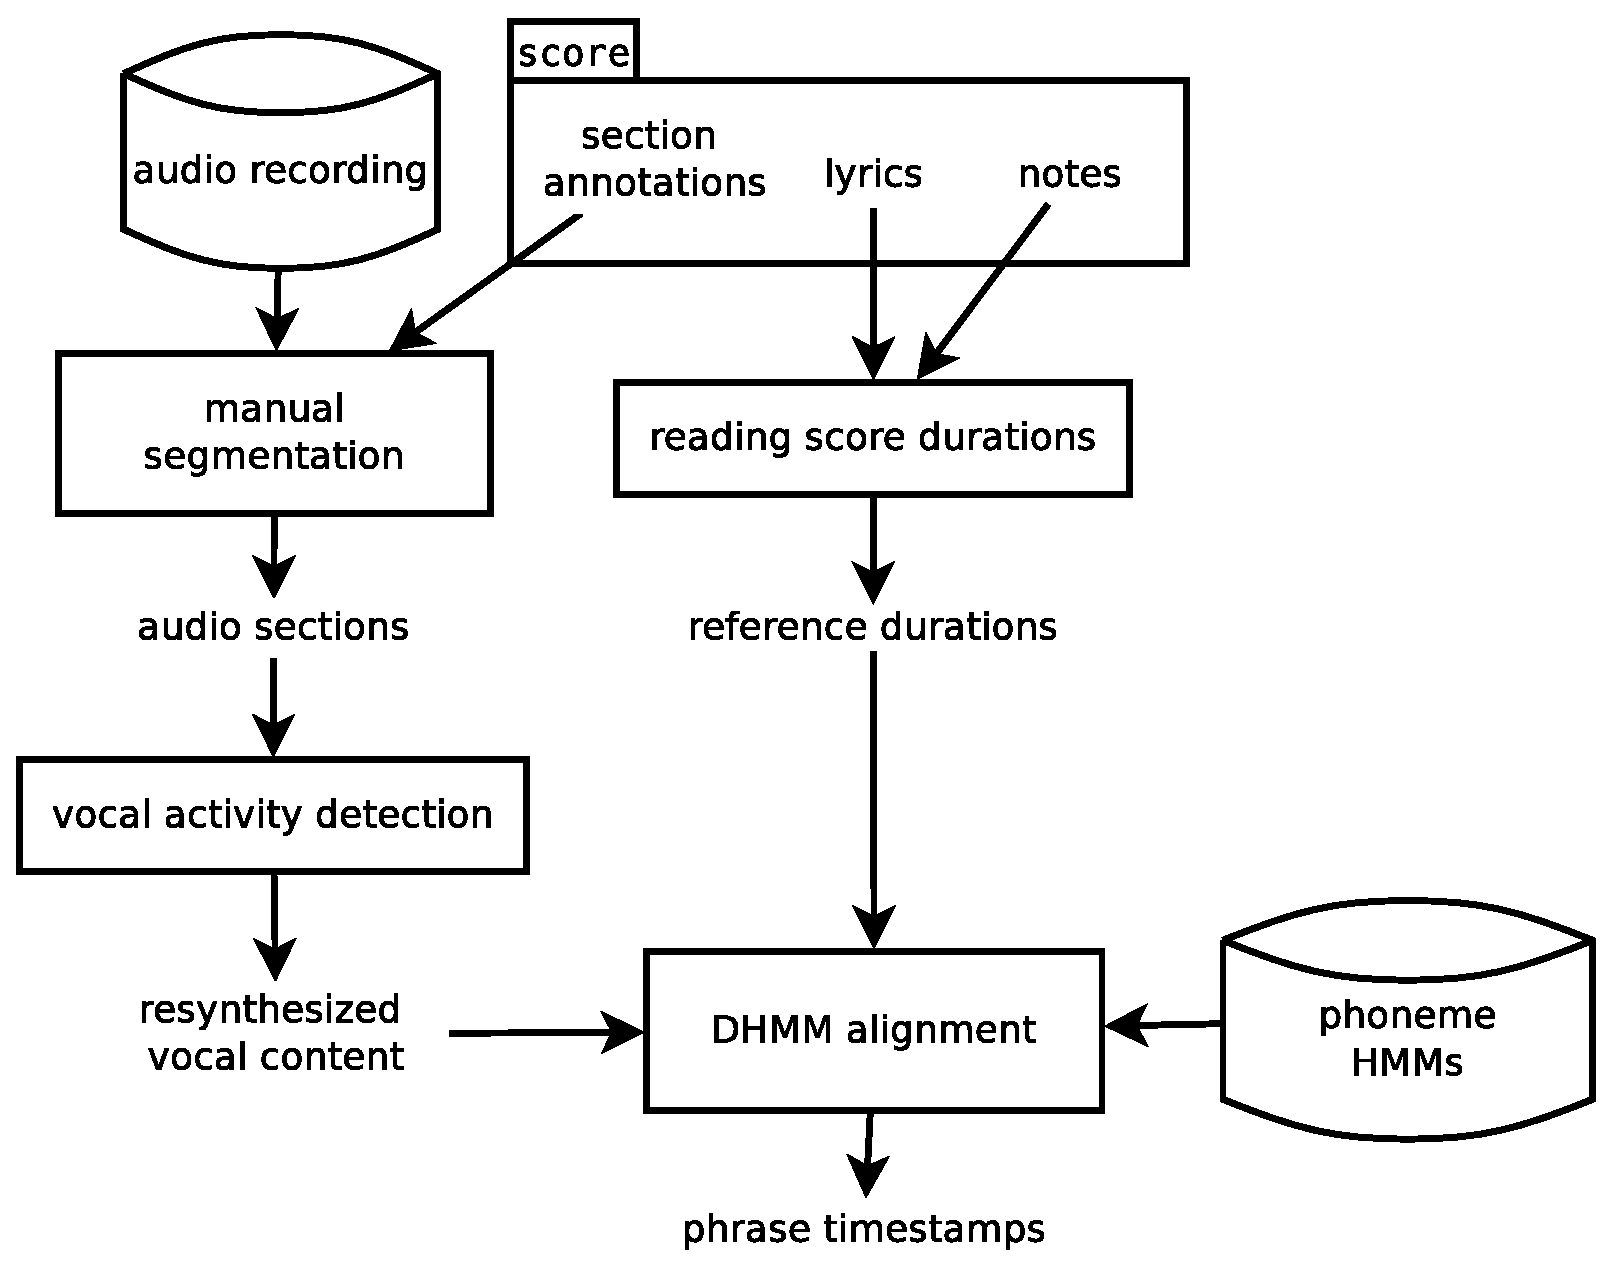
\includegraphics[width=1\columnwidth]{systemOverview}}{\small{}\medskip{}
}%
\end{minipage} \protect\caption{Overview of the modules of the proposed approach. Leftmost column
represents audio preprocessing steps, while the middle column shows
how durations are modeled. }


\label{Diagram}
\end{figure}


Similar to \cite{fujihara2011lyricsynchronizer} in this work we develop
a phoneme-recognizer-based forced alignment employing the Viterbi
algorithm \cite{rabiner1989tutorial} to decode the most optimal state
sequence. %
\begin{comment}
\textcolor{red}{TODO: more}
\end{comment}
We have adopted the idea of \cite{chen2012chord} not to explicitly
add states for durations in the model, but instead to extend the Viterbi
decoding to handle duration of states. For brevity in the rest of
the paper our model will be referred to as DHMM.

Figure \ref{Diagram} presents an overview of the proposed system.
An audio recording and its corresponding score are input. Relying
on HMMs of phonemes the DHMM returns start and end timestamps of aligned
lyrical phrases.

\textcolor{black}{First an audio recording is manually divided into
sections  (e.g. verse, chorus) as indicated in the score, whereby
instrumental-only sections are discarded. All further steps are performed
on each audio section. If we had used automatic segmentation instead,
potential erroneous lyrics and durations could have biased the comparison
of a baseline system and DHMM. As we focus on evaluating the effect
of DHMM, manual segmentation is preferred.}


\subsection{Vocal activity detection}

Next a predominant singing voice detection (a.k.a. vocal activity
detection) method \cite{salamon2012melody} is applied on each section
to attenuate the spectral content from accompanying instruments, \textcolor{black}{because
they have} negative effect on the alignment. It performs detection
of segments with predominant singing voice and in the same time melody
transcription for the detected segments. Based on the extracted melodic
contours, the vocal content is resynthesized as separate audio using
a harmonic model \cite{Serra89asystem}. This resynthesis allowed
us to perceptually evaluate the intelligibility of different vocals
after vocal detection.  More details and examples on the resynthesis
step can be found in \cite{dzhambazov2014automatic}.


\subsection{Reading score durations\label{sub:Reading-score-durations}}

For each lyrics syllable a reference duration is derived from the
values of its corresponding musical notes . \textcolor{black}{Then
the reference duration is spread among its constituent phonemes, whereby
consonants are assigned constant duration and the rest is assigned
to the vowel.}

Each phoneme is modeled by a 3-state HMM, resulting into a lookup
table of reference durations $R_{i}$ for each state $i$. We assume
that the duration $d$ for a state $i$ may vary according to a normal
distribution $P_{i}(d)$ with mean at the reference duration $d=R_{i}$
and standard deviation $\sigma$. To align a given recording the score-inferred
lengths are linearly rescaled to match its musical tempo. In this
work the unit of $R_{i}$ is number of acoustic frames. 




\subsection{Duration-explicit HMM alignment}

For each phoneme a HMM is trained from a corpus of turkish speech
utilizing MFCCs. For given lyrics, the words are expanded to phonemes
based on grapheme-to-phoneme rules for Turkish \cite[Table 1]{Salor2007580}
and the the trained HMMs are concatenated into a phoneme network.
The network is then aligned to the MFCC features, extracted from the
resynthesized audio signal, by means of the duration-explicit decoding.
In what follows we describe a variation of Viterbi decoding method,
in which maximization is carried over the most likely duration for
each state. The decoding is adapted from the procedure described in
\cite{chen2012chord}. Let us define: 
\begin{description}
\item [{$R_{max}:$}] $\max_{i}(R_{i})+\sigma$
\item [{$b_{i}(O_{t}):$}] observation probability for state $i$ for feature
vector $O_{t}$ (comply with the notation of \cite{rabiner1989tutorial})\textcolor{red}{} 
\item [{$\delta_{t}(i):$}] probability for the path with highest probability
ending in state \emph{i} at time \emph{t} (comply with the notation
of \cite[III. B]{rabiner1989tutorial}))
\end{description}



\subsubsection*{Recursion}

For $R_{max}<t\leq T$

\begin{eqnarray}
\delta_{t}(i) & = & \max_{d}\{\delta_{t-d}(i-1).\nonumber \\
 &  & P_{i}(d)^{\alpha}\thinspace[B_{t}(i,d)]^{1-\alpha}\}\label{eq:decoding}
\end{eqnarray}


where 
\begin{equation}
B_{t}(i,d)=\Pi_{s=t-d+1}^{t}b_{i}(O_{s})
\end{equation}
 is the observation probability of staying $d$ frames in state $i$
until frame $t$. The domain of $d$ comes from the normal distribution
$(\max\{R_{i}-\sigma,1\},R_{i}+\sigma)$ and is reduced for states
with reference duration $R_{i}<\sigma$. %
\begin{comment}
The recursive relateion $B_{i}(t,d+1)=$$B_{i}(t,d)\thinspace b_{i}(O_{t-d})$
allows to precompute a table and for efficient decoding
\end{comment}
\begin{comment}
IMPL: boundaries for d set in hmm.continuous.DurationPdf.DurationPdf.getMinRefDur
\end{comment}
{} %
\begin{comment}
IMPL: recursive rule eq:decoding in hmm.continuous.\_DurationHMM.\_DurationHMM.getMaxPhi
\end{comment}


A duration back-pointer is defined as
\begin{eqnarray}
\chi_{t}(i) & = & \arg\max_{d}\{\delta_{t-d}(i-1).\nonumber \\
 &  & P_{i}(d)^{\alpha}\thinspace[B_{t}(i,d)]^{1-\alpha}\}\label{eq:backpointer}
\end{eqnarray}


Note that in forced alignment the source state could be only the previous
state $i-1$. %
\begin{comment}
Thus no maximization over transition from different source states
in necessary.
\end{comment}


To be able to control the influence of the duration we have introduced
a weighting factor $\alpha$. Note that setting $\alpha$ to zero
is equivalent to using a uniform distribution for $p_{i}(d)$.

\begin{comment}
IMPL: 

instead of $\delta_{t}(i)$ we rewrite the corresponding$\phi_{t}(i)$
(to comply with the notation of Rabiner in V. A) as $\phi_{t}(i)=max_{d}\{\phi_{t-d}(i-1)+\alpha log[p_{i}(d)]+(1-\alpha)\Sigma_{s=t-d+1}^{t}log[b_{i}(O_{s})]\}$ 

and $\kappa_{t}^{'}(i)=log\pi_{i}+log[p_{i}(t)]+\Sigma_{s=1}^{t}(O_{s})$.

-----

the scaling presented in Cheng et al. is not needed since we let in
python a flag to track if there is underfllow. We divide B\_map by
its max as suggested by Cheng. 
\end{comment}


\begin{comment}
note that when d\_max(currT)<t <D\_max it might be $p_{i}(t)=0$
\end{comment}





\subsubsection*{Initialization}

For $t\leq R_{max}$

\begin{eqnarray}
\delta_{t}(i) & = & \max\{\delta_{t}(i)^{*},\thinspace\kappa_{t}(i)\}\label{eq:deltaStarOrKappa}
\end{eqnarray}
\begin{comment}
IMPL: hmm.continuous.\_DurationHMM.\_DurationHMM.\_initBeginingPhis
\end{comment}


where a reduced-duration delta $\delta_{t}(i)^{*}$ is defined in
the same way as in \eqref{eq:decoding} but 
\begin{equation}
d\in\begin{cases}
emptySet, & t\le R_{i}-\sigma\\
(R_{i}-\sigma,\min\{t-1,R_{i}+\sigma\}), & else
\end{cases}
\end{equation}
 reduces the duration to $t$ when $t<R_{i}+\sigma$. %
\begin{comment}
these boundary rules are defined in hmm.continuous.\_DurationHMM.\_DurationHMM.computePhiStar
\end{comment}


Lastly the probability of staying at initial state $i$ at time $t$
is defined as: 
\begin{equation}
\kappa_{t}(i)=\pi_{i}P_{i}(t){}^{\alpha}[\Pi_{s=1}^{t}(O_{s})]^{1-\alpha}
\end{equation}
 for $t\in(1,R_{i}+\sigma)$.

\begin{comment}
IMPL: kappa\_t(i) are computed for t in 1:R\_i + \textbackslash{}sigma,
from R\_i + \textbackslash{}sigma to R\_max + \textbackslash{}sigma
remains -infinity from initialization
\end{comment}


\begin{comment}
Python IMplementational remark:

(all indices for delta, kappa, phi as well as t are in range 0:len-1
) Only d = 1:D because d is discretized, so 0 could be a meaningful
value 
\end{comment}



\subsubsection*{}

Finally the decoded state sequence is derived by backtracking starting
at the last state $N$ and switching to a source state a number of
$d=\chi_{t}(i)$ frames ahead according to the backpointer from \eqref{eq:backpointer}.


\section{Experimental setup}

Alignment is performed on each manually divided audio section and
results are reported per recording (on total for its sections).

To assess the benefit of duration modeling for alignment a comparison
to a baseline system with standard Viterbi decoding is conducted.
We present results for the most optimal $\alpha=0.97$. It was found
by minimizing the alignment error (see section \ref{sub:Evaluation-metric})
on a separate development dataset of 20 minutes Turkish acapella recordings.
To assure optimality we aligned on word-level ground truth.

To train the speech model the HMM Toolkit (HTK) \cite{young1993htk}
is employed. The acoustic properties (most importantly the formant
frequencies) of spoken phonemes can be induced by the spectral envelope
of speech. To this end, we utilize the first 12 MFCCs and their delta
to the previous time instant.

A 3-state HMM model for each of 38 Turkish phonemes is trained, plus
a silent pause model. For each state a 9-mixture Gaussian distribution
is fitted on the feature vector. 



\textcolor{blue}{}


\subsection{Datasets}

The test dataset consists of 12 single-vocal classical Turkish music
recordings with accompaniment with total duration of \textcolor{black}{18:40
minutes}\textcolor{green}{.} Scores are provided in the machine-readable
\emph{symbTr} format \cite{karaosmanouglu2012turkish}. 

\textcolor{black}{Additionally a separate acapella dataset of the
same 12 songs sung by semiprofessional singers has been recorded especially
for this study. It can be considered a vocal-track-only version of
the original polyphonic}\textcolor{green}{{} }dataset. \textcolor{black}{Evaluation
on the acapella corpus was conducted in order to assess the impact
of the vocal extraction step.}\textcolor{red}{{} }

Each song section was manually annotated into musical phrases as proposed
by\textcolor{red}{{} \cite{karaosmanouglu2014symbolic}}. A musical
phrase usually corresponds to a lyrical line. If a phrase boundary
splits a word we have modified it to include the complete word. \textcolor{black}{Short
instrumental motives have not been excluded from the phrases. }Furthermore
we split or merged some melodic phrases so that phrases within a recording
have roughly the same number of musical bars (1 or 2). Table 1 presents
statistics about phrases. 

\begin{comment}
IMPL: final word timestamp is taken at beginning of last phoneme (assuming
it is 'sp') in Decoder.Decoder.path2ResultWordList
\end{comment}


\begin{table}
\begin{centering}
{\small{}}\global\long\def\arraystretch{1.2}
{\small{} }%
\begin{tabular}{>{\centering}p{0.25\columnwidth}>{\centering}p{0.25\columnwidth}c}
\hline 
\textbf{total\linebreak \#sections} & \textbf{\#phrases\linebreak per section} & \textbf{section duration}\tabularnewline
\hline 
{\small{}75} & {\small{} 2 to 5} & 7-20 seconds\tabularnewline
\hline 
\end{tabular}
\par\end{centering}{\small \par}

{\small{}\vspace*{-0.3cm}
 \protect\caption{Section and phrase statistics for test dataset.}
}{\small \par}

{\small{}\label{tab:dataset-stats} }%
\begin{comment}
{\small{}IMPL: file ISTANBUL/statistics}
\end{comment}
\end{table}



\subsection{Evaluation metrics\label{sub:Evaluation-metric}}

\textcolor{black}{Alignment is evaluated in terms of alignment accuracy
(AA) as the percentage of duration of correctly aligned regions from
total audio duration (see \cite[Fig.9]{fujihara2011lyricsynchronizer}
for an example). }A value of 100 means perfect matching of phrase
boundaries\textcolor{black}{. Additionally is reported the mean absolute
phrase alignment error (AE): measured at the start and end timestamp
of a phrase.}

We define a metric \emph{musical score in-sync} (MSI) to measure the
approximate degree to which a singer performs a recording in synchronization
with note values indicated in the musical score. Thus low accuracy
of MSI indicates a higher temporal deviation from musical score. We
compute\emph{ }MSI per a recording as the AA of score-inferred reference
durations $R_{i}$ (defined in section \ref{sub:Reading-score-durations})
compared to ground-truth, as if they were results after alignment.
\begin{comment}
IMPL: grThurhWordList used to compare instead of decodedWordList in
doitOneChunk.decodeAudioChunk
\end{comment}


\textcolor{red}{}




\section{Results}

\begin{table}
\begin{centering}
{\small{}}\global\long\def\arraystretch{1.2}
{\small{} }%
\begin{tabular}{>{\raggedright}p{0.38\columnwidth}>{\centering}p{0.25\columnwidth}>{\centering}p{0.25\columnwidth}}
\hline 
\textbf{\small{}System variant} & \textbf{\small{}alignment}\linebreak\textbf{\small{} accuracy}{\small{} } & \textbf{\small{}alignment}\linebreak\textbf{\small{} error}{\small{} }\tabularnewline
\hline 
musical score in-sync & 88.14 & 0.32\tabularnewline
\hline 
HMM polyphonic & 67.46 & 1.04\tabularnewline
DHMM polyphonic & 77.74 & 0.63\tabularnewline
DHMM acapella & 90.04 & 0.26\tabularnewline
\hline 
HMM+adaptation \cite{Mesaros96automaticalignment} & - & 1.4\tabularnewline
HMM+\linebreak singer adaptation \cite{fujihara2011lyricsynchronizer} & 85.2 & -\tabularnewline
\hline 
\end{tabular}
\par\end{centering}{\small \par}

{\small{}\vspace*{-0.3cm}
 \protect\caption{Alignment accuracy (in percent) for musical score in-sync; different
system variants: baseline HMM and DHMM; state-of-the-art for other
languages. Alignment accuracy is reported as total for all recordings.
Additionally the total mean phrase alignment error (in seconds) is
reported}
}{\small \par}

\label{resultsTable}
\end{table}


Table 2 presents comparison of the proposed DHMM system performance
and a baseline HMM system. It can be observed that modeling of note
values with DHMM increases HMM accuracy by 10 absolute percent. One
reason for this are cases of long vocals, in which HMM switches to
the next phoneme prematurely (due to its inability to stay long in
a given state). In contrast, the duration-explicit decoding allows
picking the optimal duration (which can be traced in an example in
figure \ref{example-of-decoded-Praat}). 
\begin{figure*}
\begin{minipage}[t]{1\columnwidth}%
\centering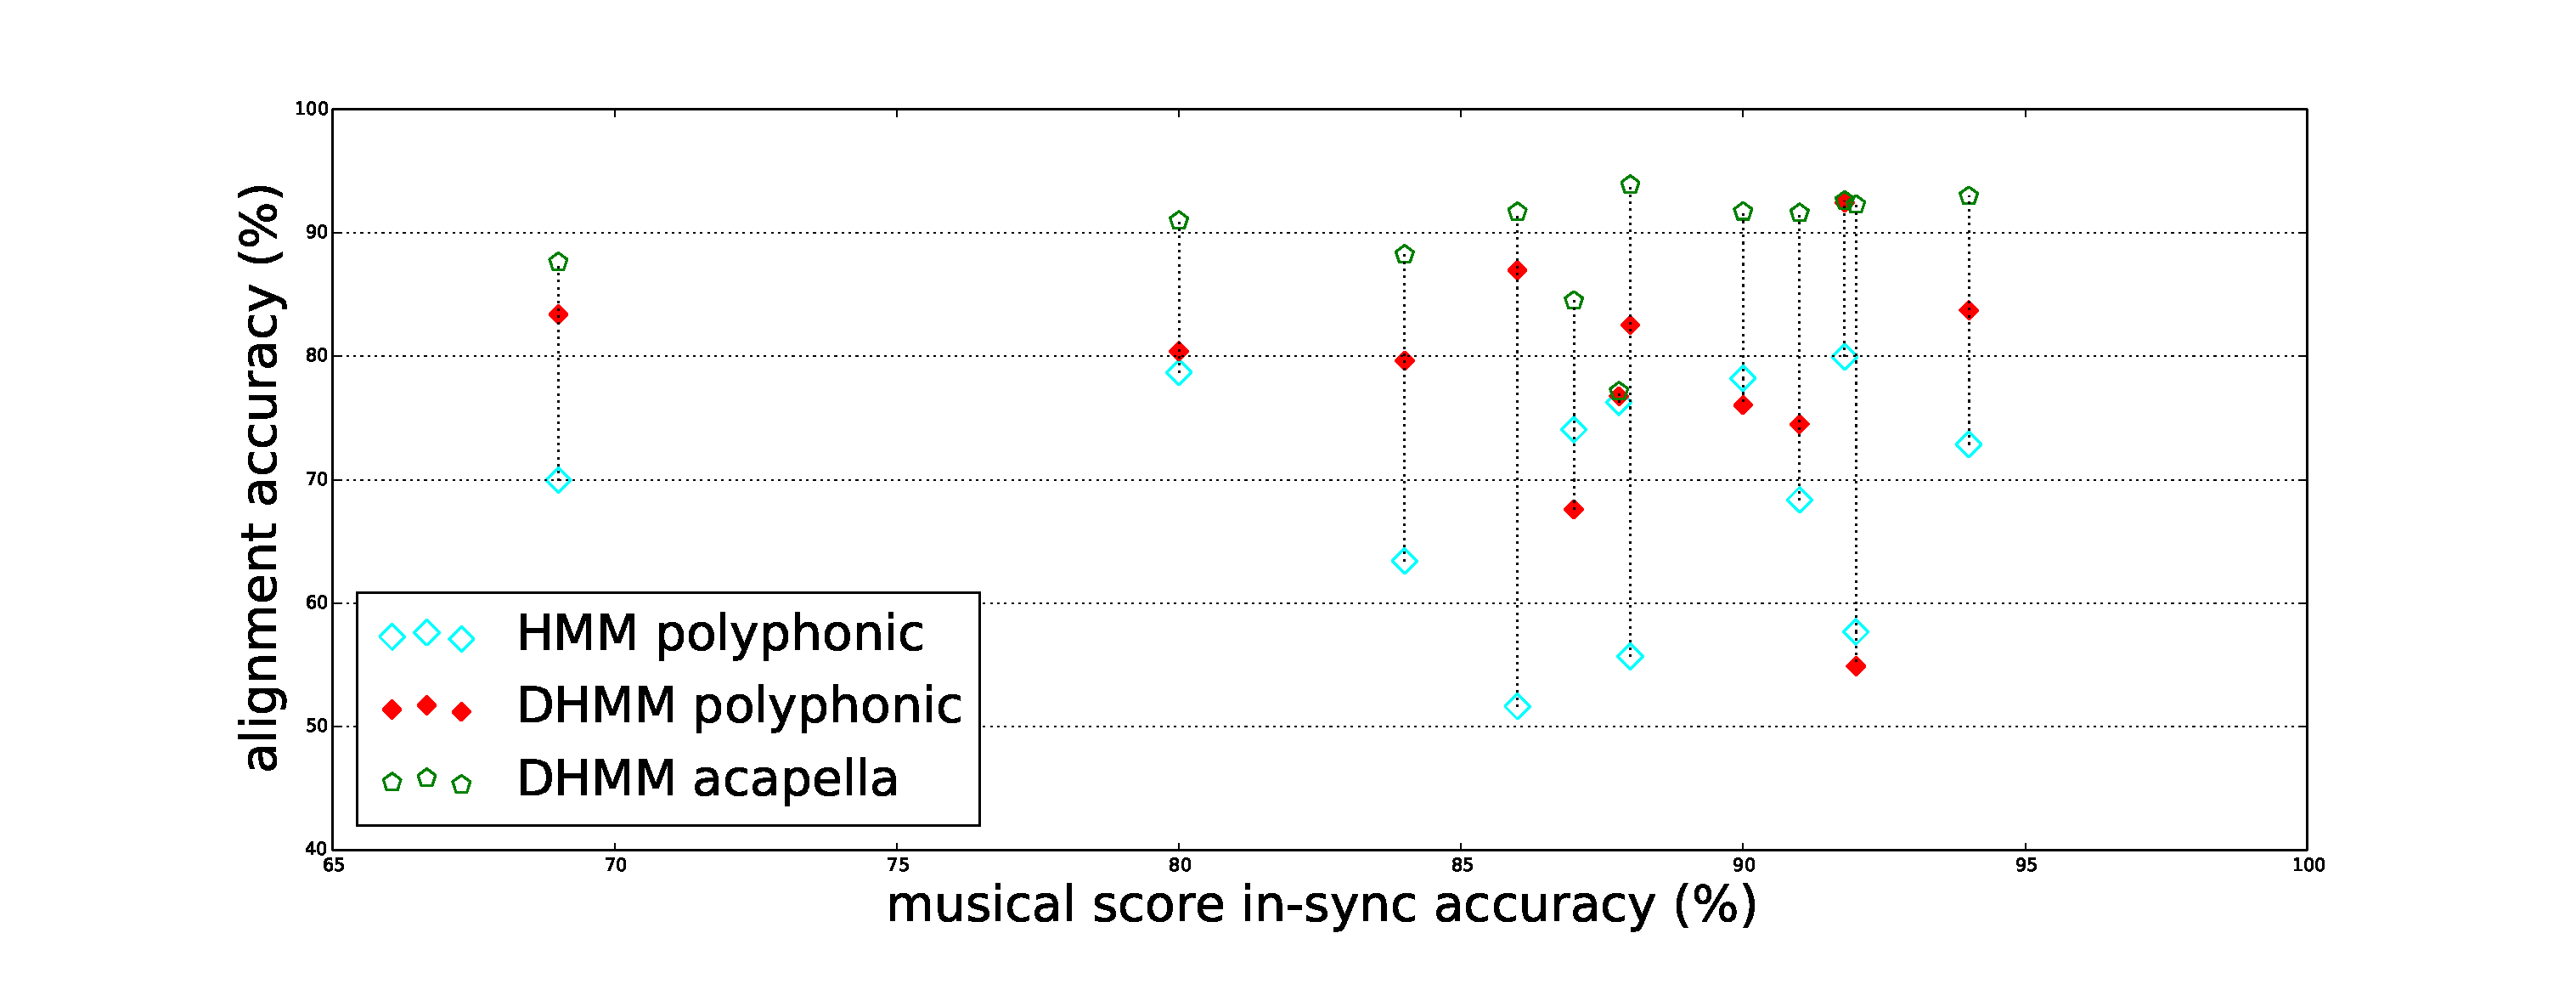
\includegraphics[width=0.8\paperwidth,height=0.3\textheight]{scatterCorrelation}%
\end{minipage}

\protect\caption{Comparison between results from DHMM (for both polyphonic and acapella)
and baseline HMM. Metric used is alignment accuracy. A connected triple
of shapes represents results for one recording. Results are ordered
according to\emph{ musical score in-sync }(on horizontal axis)}


\label{correlationGraph}
\end{figure*}


\textcolor{red}{\emph{}}%
\begin{comment}
\textcolor{red}{For experiment details see file }\textcolor{red}{\emph{experiments}}
\end{comment}
Figure \ref{correlationGraph} allows a glance at results per recording,
ordered according to MSI\emph{}%
\footnote{the per-recording results are published here \url{https://drive.google.com/file/d/0B4bIMgQlCAuqY3hKc25WTm9kTEk/view?usp=sharing}}
\emph{. }It can be observed that DHMM performs consistently better
than the baseline (with some exceptions of where accuracy is close).
Unlike the relatively stable accuracy for the acapella case, when
background instruments are present, the accuracy variates more among
recordings. 
\begin{figure}
\centering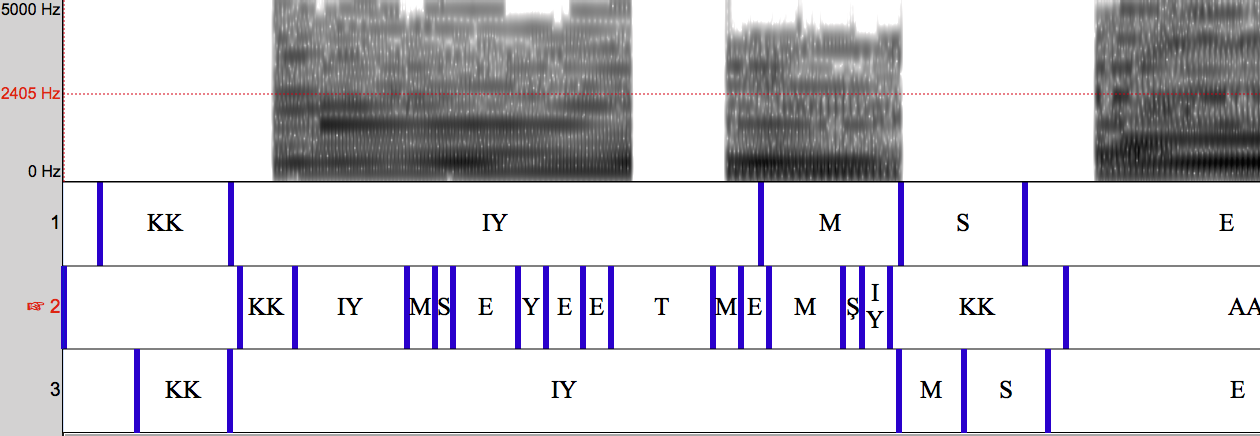
\includegraphics[width=1\columnwidth]{../DurationHSMM_polyphonic/KiseyeZeminPhoneLevel}

\protect\caption{Example of decoded phonemes. \emph{very top}: resynthesized spectrum;\emph{
upper level}: ground truth, \emph{middle level}: HMM; \emph{bottom
level}: DHMM;\emph{ }(excerpt from the recording 'Kimseye etmem \c{s}ikayet'
by Bekir Unluater)}
\textcolor{blue}{\label{example-of-decoded-Praat}}
\end{figure}


Although coming from different genre and language, we compare our
alignment results to best hitherto alignment systems for English pop
songs \cite{Mesaros96automaticalignment} and for Japanese pop \cite{fujihara2011lyricsynchronizer}.
These are abbreviated in table 2 respectively as \emph{HMM + adaptation
}and \emph{HMM + singer adaptation}. In these works alignment is evaluated
also on the \textcolor{black}{level of a lyrical line/phrase.} Except
for the duration-explicit decoding scheme, our approach differs from
both works essentially in that they conduct speech-to-singing-voice
adaptation. Unlike that we did not perform any adaptation of the original
speech model. Adaptation data of clean singing voice for a particular
singer might not always be available and thus does not allow the system
to scale to data from unknown singers. In the end, despite lacking
adaptation, our approach yields results comparable to these reference
approaches.

Moreover, \cite{fujihara2011lyricsynchronizer} trains a vocal activity
detection (VAD) module on data selected from material with same acoustics
characteristics as the test data. The VAD module showed to notably
increase the average accuracy of 72.1 \% for a baseline to accuracy
of 85.2 \% for their final system.  Similarly we observe that for
our system evaluation on the acapella dataset yields an accuracy by
about the same percent higher than the polyphonic one (see table 2).
 Investigating our results with low accuracy revealed that false
positives of our VAD module is a considerable reason for misalignment.
Unlike \cite{fujihara2011lyricsynchronizer} we did not tailor the
parameters of the VAD module used in this work (built for Western
popular music) to the specificities of our test dataset. 




\section{Conclusion}



In this work we evaluated the behavior of a HMM-based phonetic recognizer
for lyrics-to-audio alignment in two settings: with and without utilizing
lyrics duration information. Using duration-explicit modeling for
the former setting outperformed the latter for polyphonic Turkish
classical recordings. 

Importantly our approach reaches accuracy on par with state of the
art alignment systems by using an acoustic model trained on speech
only. This suggests that steps like adaptation to singing voice and
adaptation to a particular singer can be compensated by applying the
DHMM. Furthermore, the DHMM performs considerably better on an acapella
version of the test dataset, which indicates that improving the vocal
activity detection module will result in even better accuracy.

A limitation of the current alignment system is the prerequisite for
manually-done structural segmentation, which we plan to automate in
the future. 

In general, the proposed approach is applicable not only when musical
scores are available, but also for any format, from which duration
information can be inferred: for example annotated melodic contour
or singer-created indications along the lyrics.


\subparagraph*{Acknowledgements}

This work is partly supported by the European Research Council under
the European Union\textquoteright s Seventh Framework Program, as
part of the CompMusic project (ERC grant agreement 267583) and partly
by the AGAUR research grant.

% References should be produced using the bibtex program from suitable% BiBTeX files (here: strings, refs, manuals). The IEEEbib.bst bibliography% style file from IEEE produces unsorted bibliography list.% ------------------------------------------------------------------------- 

\bibliographystyle{unsrt}
\bibliography{/Users/joro/Documents/Phd/UPF/papers/FMA2014_tex_fullPaper/JabRefLyrics2Audio,/Users/joro/Documents/Phd/UPF/papers/FMA2014_tex_fullPaper/JabRefCompMusicNon-Lyrics,/Users/joro/Documents/Phd/UPF/papers/FMA2014_tex_fullPaper/JabRef_saerch_by_lyrics}

\end{document}
